% ST-DOC-01 smoke test: one-page IEEEtran conference paper.
% Purpose: verify the LaTeX toolchain (IEEEtran, TikZ, matplotlib PDF figure,
% BibTeX) of project tpu-e-cpu. Contains no project results.
% Build: latexmk -pdf -interaction=nonstopmode -halt-on-error main.tex
\documentclass[conference]{IEEEtran}

\usepackage[T1]{fontenc}
\usepackage{amsmath}
\usepackage{graphicx}
\usepackage{cite}
\usepackage{tikz}
\usetikzlibrary{positioning,arrows.meta}

% Figures generated by scripts in reports/figures/.
\graphicspath{{../../figures/}}

\begin{document}

\title{Toolchain Smoke Test for a Stochastic-Computing\\TPU Coupled to a RISC-V CPU}

\author{\IEEEauthorblockN{Author Name}
\IEEEauthorblockA{Affiliation placeholder}}

\maketitle

\begin{abstract}
This one-page document exercises the documentation toolchain of the project:
the IEEEtran conference class, an equation, a TikZ block diagram, a vector
figure produced by matplotlib, and BibTeX citations. It reports no
experimental or simulation results.
\end{abstract}

\section{Introduction}
Stochastic computing (SC) represents a value $p \in [0,1]$ as the probability
that a bit of a random stream is one~\cite{gaines1969,alaghi2013survey}.
For two independent streams $A$ and $B$, a single AND gate computes the
product
\begin{equation}
  P(A \wedge B) = P(A)\,P(B),
  \label{eq:sc_mult}
\end{equation}
which is the basic operation of an SC multiply-accumulate array.
Equation~\eqref{eq:sc_mult} is the textbook identity for independent events;
it is not a project result.
Fig.~\ref{fig:block} shows the intended top-level organisation, in which a
CPU drives the tensor processing unit (TPU) over a shared bus, and
Fig.~\ref{fig:plot} is a synthetic test plot of $y = x^2$
(CALCULATION; generator: \texttt{reports/figures/smoke\_plot.py}).

\begin{figure}[!t]
  \centering
  
\begin{tikzpicture}[
      node distance=0.9cm,
      blk/.style={draw, thick, minimum width=1.6cm, minimum height=0.8cm, align=center},
      >={Stealth[length=2mm]}]
    \node[blk] (cpu) {CPU\\(RV32I)};
    \node[blk, right=of cpu, minimum width=1.2cm] (bus) {Bus};
    \node[blk, right=of bus] (tpu) {SC-TPU};
    \draw[<->, thick] (cpu) -- (bus);
    \draw[<->, thick] (bus) -- (tpu);
  \end{tikzpicture}
  \caption{Block diagram: CPU connected to the TPU through a bus.}
  \label{fig:block}
\end{figure}

\begin{figure}[!t]
  \centering
  % evidence: reports/figures/smoke_plot.py (synthetic data, y = x^2)
  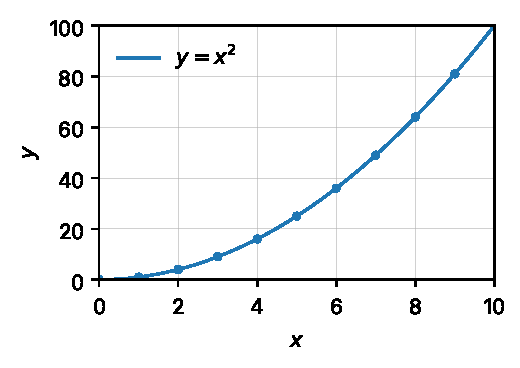
\includegraphics[width=0.9\columnwidth]{smoke_plot.pdf}
  \caption{Synthetic smoke-test plot of $y = x^2$ for $x \in [0, 10]$.}
  \label{fig:plot}
\end{figure}

\bibliographystyle{IEEEtran}
\bibliography{refs}

\end{document}
